\documentclass[10pt,a4paper,titlepage]{article}

\usepackage[a4paper]{geometry}
\usepackage{lscape}
\usepackage[utf8]{inputenc}
\usepackage[dutch]{babel}
\usepackage{enumitem}
%\usepackage[pdftex]{graphicx}

\usepackage[T1]{fontenc}
%\usepackage[ttdefault=true]{AnonymousPro}


\usepackage{multicol}
\setlength{\columnsep}{18pt}
\setlength{\columnseprule}{0pt}

\usepackage{hyperref}
\hypersetup{colorlinks,%
citecolor=black,%
filecolor=black,%
linkcolor=black,%
urlcolor=black,%
pdftex}

\usepackage{amsmath}
\usepackage{amssymb}
\usepackage{amsthm}
\usepackage{latexsym}
\usepackage{fancyhdr}
\usepackage{lastpage}
\usepackage{wrapfig}

\pagestyle{fancy}
\renewcommand{\headrule}{}
\lhead{Universiteit Leiden
}
\chead{\today}
\rhead{\thepage / \pageref{LastPage}}
\cfoot{}

\usepackage[usenames,dvipsnames]{xcolor}
\usepackage{listings}
\lstset{
	showstringspaces=false,
	columns=[l]fixed,
	keepspaces=true,
	tabsize=4,
	language=C++,
	numbers=left,
	numberstyle=\tiny,
	stepnumber=1,
	frame=leftline,
	basicstyle=\small\ttfamily,
	keywordstyle=\color{Maroon},
	commentstyle=\color{MidnightBlue}}

\usepackage{a4wide}
\usepackage{tikz}
\usetikzlibrary{arrows}
\usetikzlibrary{patterns}

\DeclareMathOperator{\bigO}{\mathcal{O}}
\DeclareMathOperator{\R}{\mathbb{R}}
\DeclareMathOperator{\N}{\mathbb{N}}
\DeclareMathOperator{\bor}{\cup}

\newcommand{\yes}{\raisebox{-1mm}{\textcolor{green!60!black}{\Checkmark}}}
\newcommand{\no}{\raisebox{-1mm}{\textcolor{red}{\XSolidBrush}}}
\newcommand{\Oh}[1]{\ensuremath{\mathcal O(#1)}}
\newcommand{\gr}[1]{\textcolor{gray}{#1}}
\renewcommand{\O}{\mathcal{O}}

\title{Team Reference Document}
\author{sudo ku
 \\ Universiteit Leiden
}


\begin{document}
%\thispagestyle{empty}
\vspace*{\stretch{1.0}}
   \begin{center}
      \Large\textbf{Team reference document}\\
      \Large\textit{sudo ku
 \\ Universiteit Leiden
}
   \end{center}
   \vspace*{\stretch{0.5}}


% Kan mooier met de tekst "Inhoudsopgave" buiten de twee kolommen, maar dat is voor later.
\begin{multicols}{2}
\tableofcontents
\end{multicols}


Deze TCR is geschreven door Raymond van Bommel $<$\url{mailto:raymondvanbommel@gmail.com}$>$, Josse van Dobben de Bruyn $<$\url{mailto:josse.vandobbendebruyn@gmail.com}$>$ en Erik Massop $<$\url{mailto:e.massop@hccnet.nl}$>$. Wij vinden het goed als anderen deze TCR gebruiken, \emph{mits} eventuele verbeteringen met ons gedeeld zijn. Ook dient tekst van gelijke strekking als deze alinea in elke versie aanwezig zijn.

\pagebreak
\section{Useful tables}

\begin{minipage}[t]{0.35\textwidth}

\begin{center}
maximale complexiteit\\
\begin{tabular}{|c|r|}
\hline
Complexiteit & max. waarde $n$\\
\hline
$\O(n!),\O(n^6)$ & 10\\
$\O(2^n\cdot n^2)$ & 15\\
$\O(n^4)$ & 100\\
$\O(n^3)$ & 400\\
$\O(n^2\lg n)$ & 2000\\
$\O(n^2)$ & 10.000\\
$\O(n\lg n)$ & 1000.000\\
$\O(n)$ & 100.000.000\\
\hline
\end{tabular}
\end{center}
\end{minipage}
\begin{minipage}[t]{0.35\textwidth}
\end{minipage}
\begin{minipage}[t]{0.35\textwidth}
\begin{center}
maximale grootte\\
\begin{tabular}{|c|r|}
\hline
data type & max. waarde\\
\hline
int & $3.27\cdot 10^4$ \\
unsigned &$6.55\cdot 10^4$ \\
long & $2.14\cdot 10^9$ \\
unsigned long&$4.29\cdot 10^9$ \\
long long& $9.22\cdot 10^{18}$ \\
unsigned long&$1.84\cdot 10^{19}$ \\
\hline
float & 7 digits\\
double & 15 digits\\
\hline
\end{tabular}
\end{center}
\end{minipage}
\begin{minipage}[t]{0.3\textwidth}
\begin{center}Machten van 2\\
\begin{tabular}{|c|r|}
\hline
2-macht & dec. waarde\\
\hline
$2^{10}$ & $1,02\cdot10^3$\\
$2^{20}$ & $1,04\cdot10^6$\\
$2^{30}$ & $1,07\cdot10^9$\\
$2^{40}$ & $1,10\cdot10^{12}$\\
$2^{50}$ & $1,13\cdot10^{15}$\\
$2^{60}$ & $1,15\cdot10^{18}$\\
\hline
\end{tabular}
\end{center}
\end{minipage}

%TODO complexitiet van veelgebruikte (deel)algoritmes


%\section{Setup}
\iffalse
\subsection{Bestand ``name.cpp''}
\begin{multicols}{2}
\lstinputlisting{parts/name.cpp}
\end{multicols}
\fi

\iffalse
\subsection{Bestand ``Makefile''}
\lstinputlisting[language=make]{parts/Makefile}

\subsection{Bestand ``setup.sh''}
Maak eerst een \textbf{backup} van reeds bestaande bestanden! Better be safe than sorry.
\lstinputlisting[language=bash]{parts/setup.sh}
\fi

\iffalse
\section{Binary Search}

Deze implementatie zorgt dat \verb|lo| steeds in het `toegestane' gebied zit en \verb|hi| in het `verboden' gebied. In het begin stellen we ze op ongeldige waarden in. Dat maakt niet uit, want als hierdoor \verb|mid| op een ongeldige waarde uitkomt, dan schelen \verb|lo| en \verb|hi| maar 1 en waren we al buiten de lus. We retourneren de hoogste index die mag.
\begin{lstlisting}
lo = -1; // 1 voor begin
hi = N; // 1 na begin
while (hi-lo > 1) {
	mid = (lo+hi)/2;
	(mag (mid) ? lo : hi) = mid;
}
return lo;
\end{lstlisting}
\fi

\section{Bomen}
\iffalse
\subsection{Fenwick tree}

Het array is 1-based. Er geldt \verb.LSONE(i) = i & (-i). Bij updaten: zolang \verb.i <= n., update \verb.s[i]. en \verb.i += LSOne(i).. Bij sommeren: zolang \verb.i >= 0., tel \verb.f[i]. bij het antwoord op en doe \verb.i += LSOne(i)..

\fi
\iffalse
\[
\underbrace{
\underbrace{\underbrace{\underbrace{a[0]}_{f[0]} a[1]}_{f[1]} \underbrace{a[2]}_{f[2]} a[3]}_{f[3]}
\underbrace{\underbrace{a[4]}_{f[4]} a[5]}_{f[5]} \underbrace{a[6]}_{f[6]} a[7]}_{f[7]}
\underbrace{\underbrace{\underbrace{a[8]}_{f[8]} a[9]}_{f[9]} \underbrace{a[10]}_{f[10]} a[11]}_{f[11]}
\underbrace{\underbrace{a[12]}_{f[12]} a[13]}_{f[13]} \underbrace{a[14]}_{f[14]}.
\]

Bedenkend dat \lstinline{i |= i+1} de minst-significante 0 van $i$ op 1 zet, en dat \lstinline{k &= k-1} de minst-significante $1$ van $k$ op 0 zet, vinden we deze code:
\lstinputlisting{parts/fenwick.cpp}

Voor gerelateerde toepassingen kan het makkelijker zijn om een binaire boom met $2n-1$ knopen en $n$ bladeren te gebruiken.
\fi

\subsection{Segment tree}
Onderstaande code werkt voor het dynamische Range Minimum Query probleem. Range updates kunnen worden geimplementeerd met lazy propagation: houd bij of een segment volledig naar een bepaalde waarde ge\"updated moet worden.
\lstinputlisting{parts/segmenttree.cpp}

\subsection{Fenwick tree}
\lstinputlisting{parts/fenwick.cc}

\subsection{Minimal spanning tree}

%\subsubsection{Kruskals algoritme}

\lstinputlisting{parts/kruskal.cpp}
Voor een efficiënte implementatie van \lstinline{init}, \lstinline{merge} en \lstinline{representant} is een of andere Disjoint-Set datastructuur handig. 

\subsection{UFDS}
Een Disjoint-Set Forest (met amortized $\bigO(\alpha(n))$-tijd per operatie, met $\alpha$ de inverse van de Ackermann functie):
\lstinputlisting{parts/unionfind.cpp}

\iffalse
\subsection{Kosaraju's algoritme voor SCC's}
For each vertex u of the graph, mark u as unvisited. Let L be empty. For each vertex u of the graph do Visit(u), where Visit(u) is the recursive subroutine:
\begin{verbatim}
If u is unvisited then:
Mark u as visited.
For each out-neighbour v of u, do Visit(v).
Prepend u to L.
Otherwise do nothing.
\end{verbatim}
For each element u of L in order, do Assign(u,u) where Assign(u,root) is the recursive subroutine:
\begin{verbatim}
If u has not been assigned to a component then:
Assign u as belonging to the component whose root is root.
For each in-neighbour v of u, do Assign(v,root).
Otherwise do nothing.
\end{verbatim}
\fi


\section{Grafen}

\subsection{Depth First Search}

DFS heeft vele toepassingen. Bij sommige van deze dingen willen we knopen als actief danwel gedaan markeren. Dan kunnen we ook buren overslaan.
\begin{itemize}[noitemsep,nolistsep]
\item Gerichte cykels: als een reeds actieve knoop wordt ontwikkeld.
\item Ongerichte cykels: als een reeds actieve, of voltooide knoop wordt ontwikkeld.
\end{itemize}

($\bigO(V+E)$ en $\bigO(V^2)$)
\begin{lstlisting}
vector<vi> AdjList //Adjacency list

vi dfs_num; //set all values to UNVISITED
void dfs(int u){
ii v;
dfs_num[u] = VISITED;
for(int j = 0; j < AdjList[u].size(); j++){
v = AdjList[u][j];
if (dfs_num[v] == UNVISITED){
dfs(v);DFS
}	}	}
\end{lstlisting}

\subsection{Breadth first search}
($\bigO(V+E)$ en $\bigO(V^2)$)

\begin{lstlisting}
vector<vi> AdjList //Adjacency list
vi d(V, INF); d[s] = 0;
queue<int> q; q.push(s);
int u,v;
while(!q.empty()){
u = q.front(); q.pop(); // get the first element from our queue
for(int j = 0; j < AdjList[u].size(); j++){
v = AdjList[u][j]
if(d[v] == INF){ //test if unvisited
d[v] = d[u] + 1; //mark our visit
q.push(v);
}	}	}
\end{lstlisting}


\subsection{Topologisch sorteren}

Laat de globale variabele \texttt{n} het aantal punten van een graaf zijn.
De volgende code registreert de finishvolgorde van de knopen in een globale variable \lstinline{vector<int> finished}. Hiermee is $\text{\lstinline{finished[n-1]}} < \cdots < \text{\lstinline{finished[0]}}$ een topologische sortering van de knooppunten.

\subsection{2-SAT}

De code gaat ervanuit dat er \lstinline{n} knopen zijn, waarbij knopen $2i$ en $2i+1$ elkaars negatie zijn. De functie retourneert of er een oplossing is. Als er een oplossing is, dan is \lstinline{val[comp[i]]} de valuatie van knoop $i$ in een oplossing.

\subsection{Code 2-SAT, SCC en DFS}
\lstinputlisting{parts/2satgraph.cpp}
\lstinputlisting{parts/dfs.cpp}
\lstinputlisting{parts/finishsort.cpp}
\lstinputlisting{parts/scc.cpp}
\lstinputlisting{parts/2sat.cpp}


\subsection{Biconnected components}

De volgende code deelt de takken van de graaf op in componenten die verbonden blijven als er 1 knoop verwijderd wordt. In het commentaar staat hoe je de punten bepaald die de graaf splitsen als je ze verwijderd.

\lstinputlisting{parts/bicon.cpp}

\subsection{Kortste pad}

\subsubsection{Dijkstra's algoritme}

Dijkstra's algoritme werkt alleen voor grafen met niet-negatieve gewichten.
%\lstinputlisting{parts/dijkstranieuw.cc}
%In principe kan een knoop met ingraad $i$ hier $i$-maal aan de priority-queue worden toegevoegd. 
Een korte implementatie die knopen meerdermaals aan de PQ toe kan voegen is:
\lstinputlisting{parts/dijkstrakort.cc}
Deze implementatie hoort ook te werken met negatieve gewichten, hoewel langzamer. Pas wel op voor negatieve cycels!
met eigen ordening:
\begin{lstlisting}
struct Order
{
    bool operator()(ii const& a, ii const& b) const
    {
        return a.first > b.first;//or any other ordering
    }
};
//...
priority_queue<ii, vector<ii>, Order > pq;
\end{lstlisting}

\subsubsection{Negatieve cykels}
Bellman-Ford: relax elke edge $V$ keer (makkelijk te implementeren met edge list). Negatieve-cykeldetectie: kijk of er na het uitvoeren nog iets te relaxen valt.

Kan ook met Floyd-Warshall/

Nota Bene: deze implementatie ondersteunt slechts paden van hoogstens \lstinline{INT_MAX/4} !

\lstinputlisting{parts/bellmanford.cpp}

\subsubsection{Floyd-Warshall}
Floyd-Warshall vindt de lengtes van de paden van elke knoop naar elke andere knoop.

\begin{lstlisting}
for k = 1 to n {
	for i = 1 to n {
		for j = 1 to n {
			dist[i][j] = min (dist[i][j], dist[i][k] + dist[k][j]);
		}
	}
}
\end{lstlisting}

%TODO wellicht een leuk idee om ook Bellman-Ford hier neer te zetten

\iffalse
\subsubsection{Afwijkende applicaties}
Een aantal andere problemen is op te lossen met (aanpassingen van) kortste pad algoritmen:

\begin{itemize}[noitemsep,nolistsep]
\item Vind het pad met de maximale capaciteit tussen $S$ en $T$. De capaciteit is het minimum van de capaciteiten van de kanten in het pad.

We passen het algoritme van Dijkstra aan. We kiezen nu telkens het punt met maximale capaciteit, in plaats van het punt met minimale afstand. Het is niet zinnig om hiervoor Bellman-ford te gebruiken.

\item Een soortgelijke aanpassing van het kortste pad probleem kan gebruikt worden om een pad met een maximale waarschijnlijkheid/betrouwbaarheid/... te vinden. Oftewel een pad waarbij ``waarde'' het product is van de gewichten van de kanten. Vervang elk gewicht $w$ door $-\log(w)$. Merk op dat voor waardes groter dan $1$ deze afstanden negatief kunnen worden.

\end{itemize}

\fi

\subsection{Flow netwerken}

\lstinputlisting{parts/flowgraph.cpp}
 
 Als je vanaf het begin al takken met negatieve kosten en strikt positieve capaciteit hebt moet je \texttt{potential} initialiseren met Bellman-Ford. Dit algoritme ondersteunt geen negatieve cykels.
 
\subsection{Max-flow}
De Edomond-Karp implementatie van Ford-Fulkerson (mbv BFS)
\lstinputlisting{parts/edmond-karp(maxflow).cpp}
\subsection{Min-cut}
Als je na max-flow kijk naar alle knopen die je kan berijken vanaf de scoure via positieve ($\not=0$) takken kan bereiken, heb je een min-cut
De min-cut wordt ge\"{i}nduceerd door de verzameling punten die bereikbaar zijn vanuit de bron. Bedenk dat dit in principe al in de mark array staat na \texttt{ford\_fulkerson}.

\section{Computational Geometry}

\subsection{Geometry}
%\lstinputlisting{parts/geom.cpp}
\lstinputlisting{parts/geom_lines.cc}

\subsection{Projecties}
\lstinputlisting{parts/dot.cpp}
De projectie $p(x,y)$ van $x\in\R^n$ op $y\in\R^n$ wordt gegeven door:
\[ \text{$p(x,y) = \frac{x\cdot y}{|y|}\hat{y} = \frac{x\cdot y}{|y|^2}y = \frac{x\cdot y}{y\cdot y}y$, ~~~~ waarbij $\hat{y} = \frac{y}{|y|}$.}\]
Dit is een scalair veelvoud van $\hat{y}$. Let op dat $x\cdot y$ een inproduct is en geen scalair product!

\subsection{Rotaties}
Om een vector $(x,y)\in\R^2$ precies $\theta$ graden in positieve richting te draaien:
\begin{align*}
	\begin{pmatrix}
		x' \\
		y'
	\end{pmatrix} = \begin{pmatrix}
		\cos(\theta) & -\sin(\theta) \\
		\sin(\theta) & \cos(\theta)
	\end{pmatrix}\begin{pmatrix}
		x \\
		y
	\end{pmatrix}.
\end{align*}


\begin{wrapfigure}{r}{.34\textwidth}
	\centering
	\vspace{-1cm}
	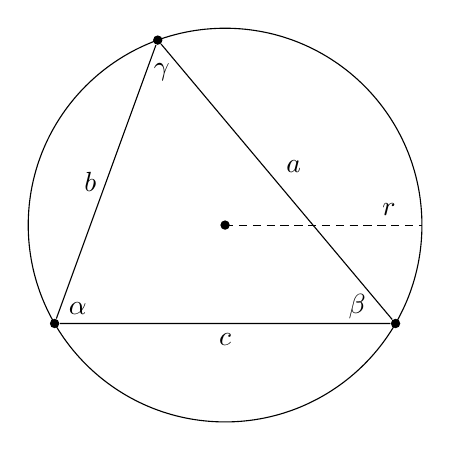
\begin{tikzpicture}[punt/.style={fill,circle,inner sep=1.2pt},scale=2.5]
		\node[punt] (A) at (210:1cm) {};
		\node[punt] (B) at (330:1cm) {};
		\node[punt] (C) at (110:1cm) {};
		\node at (209.5:8.6mm) {$\alpha$};
		\node at (328.2:7.9mm) {$\beta$};
		\node at (112.5:8.4mm) {$\gamma$};
		\draw (0,0) circle (1cm);
		\draw (A) -- node[below] {$c$} (B) -- node[above right] {$a$} (C) -- node[left] {$b$} (A);
		\node[punt] at (0,0) {};
		\draw[densely dashed] (0,0) -- node[near end,above right] {$r$} (1,0);
	\end{tikzpicture}
\end{wrapfigure}
\iffalse
\subsection{Sinusregel, cosinusregel, tangensregel}
In iedere driehoek geldt:
\[ \frac{a}{\sin(\alpha)} = \frac{b}{\sin(\beta)} = \frac{c}{\sin(\gamma)} = 2r. \]
Ook geldt:
\[ c^2 = a^2 + b^2 - 2ab\cos(\gamma) \]
en
\[ \frac{a - b}{a + b} = \frac{\tan(\frac{1}{2}(\alpha - \beta))}{\tan(\frac{1}{2}(\alpha + \beta))}. \]

\subsection{Hoekformules}

Er geldt voor het inproduct dat 
\[
p \cdot q  = |p||q|\cos(\theta)
\]
met $\theta$ de hoek tussen de vectoren. Voor het uitproduct geldt dat
\[
p \times q = |p||q| \sin(\theta) \ n
\]
met $n$ de genormaliseerde normaal.


\subsection{Uit-product}
\lstinputlisting{parts/cross.cpp}
Het uitproduct $p\times q = \det\left(\begin{smallmatrix}x_1 & x_2\\y_1 & y_2\end{smallmatrix}\right) = x_1y_2 - x_2y_1 = -q\times p$ is gelijk aan de oppervlakte van het parallellogram ge\"induceerd door $p_1$ en $p_2$ (zie figuur (a)).

\smallskip

\begin{center}
	\newcommand{\akeerb}{\textcolor{blue}{p}\;\textcolor{black}{\times}\;\textcolor{red}{q}}
	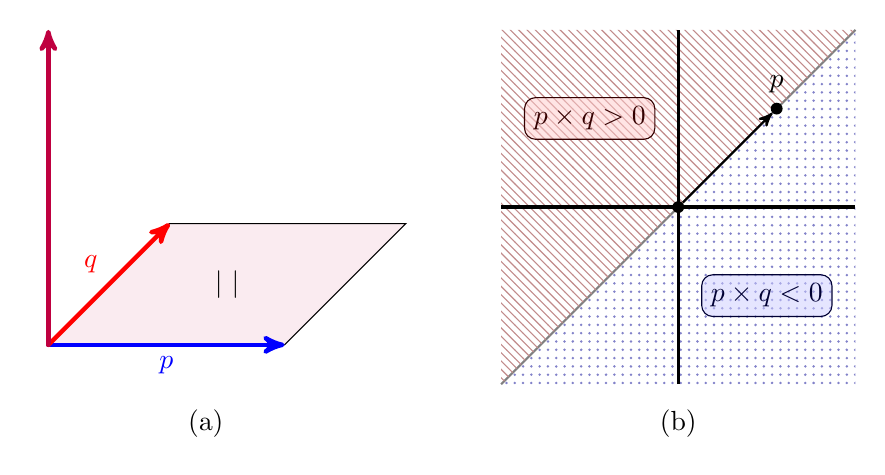
\begin{tikzpicture}[>=stealth',
	                    punt/.style={circle,fill,inner sep=0pt,minimum height=1.5mm},
	                    blok/.style={draw=black,rectangle,rounded corners,fill=white,fill opacity=0.5,draw opacity=1,text opacity=1}]
		\fill[draw,fill=purple!8!white] (0,0,0) -- (3,0,0) -- (3,0,-4) -- (0,0,-4) -- (0,0,0);
		\begin{scope}[line cap=round,->,>=stealth']
			\draw[ultra thick,blue] (0,0,0) to node[below] {$p$} (3,0,0);
			\draw[ultra thick,red] (0,0,0) to node[above left] {$q$} (0,0,-4);
			\draw[ultra thick,purple] (0,0,0) to node[left] {$\akeerb$} (0,4,0);
		\end{scope}
		\node at (1.5,0,-2) {$|\,\akeerb\,|$};
		
		\node at (2,-1) {(a)};
		
		\begin{scope}[xshift=8cm,yshift=1.75cm]
			\coordinate (nw) at (-2.25, 2.25);
			\coordinate (no) at ( 2.25, 2.25);
			\coordinate (zw) at (-2.25,-2.25);
			\coordinate (zo) at ( 2.25,-2.25);
			\draw[thick,gray] (zw) -- (no);
			\fill[pattern=north west lines,pattern color=red!30!gray!70] (nw) -- (no) -- (zw);
			\fill[pattern=dots,pattern color=blue!40!gray!70] (zo) -- (no) -- (zw);
			
			\draw[very thick] (-2.25,0) -- (2.25,0) (0,-2.25) -- (0,2.25);
			\node (D) [punt] at (0,0) {};
			\node (E) [punt] at (1.25,1.25) [label=above:$p$] {};
			\draw[thick,->] (D) -- (E);
			
			\node[blok,red!20!black,fill=red!20!white] at (-1.125,1.125) {$p\times q > 0$};
			\node[blok,blue!20!black,fill=blue!20!white] at (1.125,-1.125) {$p\times q < 0$};
			
			\node at (0,-2.75) {(b)};
		\end{scope}
	\end{tikzpicture}
\end{center}


In de $\mathbb{R}^3$ is het uitproduct:

\[
\left( \begin{array}{r} x_1 \\ y_1 \\ z_1 \end{array} \right) \times  \left( \begin{array}{r} x_2 \\ y_2 \\ z_2 \end{array} \right) = 
\left( \begin{array}{r} 
y_1z_2 - y_2z_1 \\
z_1x_2 - z_2x_1 \\
x_1y_2 - x_2y_1
\end{array} \right)
\]


\subsubsection{Hoek tussen vectoren}
Het teken van $p\times q$ vertelt ons iets over de hoek tussen de vectoren $p$ en $q$ (zie figuur (b)).
\begin{itemize}[noitemsep,nolistsep]
	\item Als $q$ in positieve richting (tegen de klok in) van $p$ ligt, geldt $p\times q > 0$.
	\item Als $q$ in negatieve richting (met de klok mee) ligt, geldt $p\times q < 0$.
	\item Als $p$ en $q$ dezelfde hoek hebben (modulo $180^\circ$), geldt $p\times q = 0$. In dit geval is $p$ een re\"eel veelvoud van $q$ of andersom.
\end{itemize}

\subsubsection{Bocht naar links of rechts?}
\lstinputlisting{parts/direction.cpp}
Bepalen of de aaneengesloten vectoren $\overrightarrow{p_1p_2}$ en $\overrightarrow{p_2p_3}$ een bocht naar links of rechts maken in $p_2$:
\begin{itemize}[noitemsep,nolistsep]
	\item Als $(p_2 - p_1)\times (p_3 - p_1) > 0$ geldt, dan is de bocht naar links.
	\item Als $(p_2 - p_1)\times (p_3 - p_1) < 0$ geldt, dan is de bocht naar rechts.
	\item Als $(p_2 - p_1)\times (p_3 - p_1) = 0$ geldt, dan is er geen bocht.
\end{itemize}

\fi

\subsubsection{Snijden twee lijnstukken?}
Er zijn een paar vervelende randgevallen. Onderstaande code (functie \texttt{segmentsIntersect}) werkt. Deze functie onderzoekt of de lijnstukken $\overrightarrow{p_1p_2}$ en $\overrightarrow{p_3p_4}$ elkaar snijden. De code werkt ook als de co\"ordinaten in \texttt{float} of \texttt{double} zijn.

\lstinputlisting{parts/intersect.cpp}

%TODO \subsection{Sweepline}
\subsection{Oppervlakte van een veelhoek}
\[
\text{opp} = \frac{1}{2} \left| \quad \sum_{(x,y) \rightarrow (x', y') \in A} xy' - x'y \quad \right|
 \]


\subsection{Zwaartepunt van een veelhoek}

Het zwaartepunt kan bepaald worden met
\[
C_x = \frac{1}{6A} \sum_{(x,y)\to(x',y')} (x+x')(xy' - x'y)
\]
En 
\[
C_y = \frac{1}{6A} \sum_{(x,y)\to(x',y')} (y+y')(xy' - x'y)
\]
Met $A$ de oppervlakte van de veelhoek.
Deze methode werkt niet als de veelhoek zichzelf doorsnijdt.

\subsection{Polygon}

\lstinputlisting{parts/poly.cc}

\iffalse
%Deze code produceert uit \lstinline{vector<punt> punten}
 een lijst van halfopen zijden van de convex hull, waarbij de hoekpunten steeds als laatste punt in de zijde voorkomen.
Zo geeft $\text{punten} = \{(x,y) : 1 \leq x \leq y \leq 3\}$ een cyclische permutatie van
\[
[[(1,1), (0,0)], [(1,0), (2,0)], [(2,1), (2,2)]] \quad\text{of}\quad
[[(0,1), (0,0)], [(1,1), (2,2)], [(2,1), (2,0)]],
\]
afhankelijk van de richting waarin de convex hull afgelopen wordt.
Algoritme werkt niet betrouwbaar als punten meerdere keren voorkomen.
Algoritme werkt niet als het aantal punten $1$ of minder is.
Als alle punten op een lijn liggen, dan krijgen we eindpunten eenmaal en interne punten tweemaal.
\lstinputlisting{parts/graham.cpp}
\fi

%\subsection{Calipers}
%\lstinputlisting{parts/calipers.cc}
\iffalse
\subsection{Snijpunten bepalen}

\subsubsection{Cirkel-Cirkel}

\lstinputlisting{parts/circles_intersect.cpp}


\subsection{Closest pair of points}

\lstinputlisting{parts/closest.cpp}

%TODO \subsubsection{Jarvis march}
\fi

\section{Dynamic Programming}
\subsection{Knapsack}
\lstinputlisting{parts/knapsack.cc}
%TODO \subsection{Memoization}
%TODO \subsection{Longest decreasing subsequence}

%TODO \section{Linear Programming}

\section{Strings} 

\subsection{String Matching}

\lstinputlisting{parts/kmp.cpp}
\iffalse
\subsection{Multistring matching}

\lstinputlisting{parts/ahocorasick.cpp}
\fi
\iffalse
\subsection{Suffix Array}

De volgende code kan de suffix array van een string bepalen en de least commmon parent oftwel de lengte van de gemeenschappelijke prefix van twee suffixes bepalen.

\lstinputlisting{parts/suffix_array.cpp}

\subsection{Suffix Tree}

\lstinputlisting{parts/ukkonen.cpp}

\subsection{Longest common subsequence}

De uitdrukking $c[i,j]$ hieronder is de lengte van de longest common subsequence van strings $x_1\cdots x_i$ en $y_1\cdots y_j$:
\[ c[i,j] = \left\{\begin{array}{ll}
0 & \text{als $i = 0$ of $j = 0$} \\
c[i-1][j-1] + 1 & \text{als $i > 0$ en $j > 0$ en $x_i = y_j$} \\
\max (c[i,j-1], c[i-1,j]) & \text{als $i > 0$ en $j > 0$ en $x_i \neq y_j$}
\end{array}\right. .
 \]

\subsection{Longest increasing subsequence}
\lstinputlisting{parts/lis.cpp}
\fi

\subsection{Levenšteinafstand}
Het minimal aantal operaties nodig om een string in een andere te transformeren, met toegestane operaties invoeging, verwijdering en subsitutie van karakters. Hieronder is de expressie $d[i,j]$ de Levenšteinafstand tussen $x_1\cdots x_i$ en $y_1\cdots y_j$:
\[ d[i,j] = \left\{\begin{array}{ll}
i+j & \text{als $i = 0$ of $j=0$} \\
\min\left(\begin{array}{c}d[i-1,j]+1,\\ d[i,j-1]+1,\\ d[i-1,j-1] + 1_{\{x_i \neq y_j\}}\end{array}\right) & \text{als $i > 0$ en $j>0$}
\end{array}\right.
\]


\section{Getaltheorie}
\subsection{Priemgetallen}
\lstinputlisting{parts/primes.cc}


\subsection{Uitgebreide Euclidische algoritme}
Met dit algoritme kan zowel de ggd van twee getallen $a$ en $b$ bepaald worden als een paar $(x,y)$ waarvoor geldt $ax + by = \textrm{ggd}(a,b)$.

\begin{minipage}{0.5\textwidth}
\lstinputlisting{parts/uggd.cpp}
\end{minipage}
\begin{minipage}{0.5\textwidth}
\lstinputlisting[frame=btlr]{parts/ggd.cpp}
\end{minipage}

\subsection{CRT}
\lstinputlisting{parts/crt.cc}

\subsection{Priemtest}

De volgende code implementeert een deterministische versie van Miller-Rabin:

\lstinputlisting{parts/isprime.cpp}

Dit gebruiken we om te voorkomen dat we grote priemgetallen in Pollards-Rho gaan gooien
\lstinputlisting{parts/Pollardsrho.cpp}

\subsection{Partitiefunctie}

De partitiefunctie geeft het aantal manieren dat een getal $n$ opgedeeld kan worden in positieve getallen als volgorde niet uitmaakt, zodanig dat de som weer $n$ is.

\begin{minipage}{0.7\textwidth}
\lstinputlisting{parts/partition.cpp}
\end{minipage}
\begin{minipage}{0.3\textwidth}
\textbf{Overflow}

\begin{tabular}{|r|r|} \hline
type & iteraties veilig \\ \hline
s32 & $121$ \\ \hline
u32 & $127$ \\ \hline
s64 & $405$ \\ \hline
u64 & $416$ \\ \hline
s128 & $1437$ \\ \hline
u128 & $1458$ \\ \hline
\end{tabular}
\end{minipage}


\section{Lineaire stelsels oplossen}

We kunnen een stelsel lineaire vergelijkingen oplossen met het vegen van een matrix. De volgende code doet dat als de matrix inverteerbaar is en geeft \texttt{false} als de matrix niet inverteerbaar is.

\lstinputlisting{parts/linsolve.cpp}
\iffalse
\subsection{Determinant berekenen}

We kunnen de determinant van een matrix bepalen door via Gauss-eliminatie een matrix te maken waarvan alles onder de diagonaal $0$ is. Vervolgens nemen we het product van de diagonaal en dat is dan de determinant. Let op dat hoewel het optellen van rijen de determinant niet veranderd, het schalen dat wel doet en dat je dus in het bijzonder niet alle pivots naar $1$ moet normaliseren. 
\fi
\iffalse
\section{Fourier Transformatie}

\subsection{complexe Fourier Transformatie}

Neem al aan dat de inputgrootte een macht van $2$ is. Bij gebruik voor integers  gebruik \verb-round- voor conversie.

\lstinputlisting{parts/fft.cpp}
\fi

\begin{multicols}{2}
[
\section{Tips}
]
\subsection{Mogelijke algoritmes, inspiratie}
\begin{itemize}[noitemsep,nolistsep]
\item Probeer te denken vanuit de grenzen. 
\item Is het te doorzoeken met min/max binair/ternair zoeken? (monotoon?)
\item Brute Force (met pruning)
\item Brute Force small instances to discover patterns or test algorithm
\item Probeer Greedy
\item Dynamic Programming
\item (Mincost)Maxflow
\item longest increasing subsequence
\item Kan je de graaf bipartiet krijgen?
\item Precalculeren
\item Inclusion/Exclusion
\item Neigt het naar NIM?
\item Line sweep / radial sweep
\item Coordinaten comprimeren
\item Vervang strings met iets snellers.
\end{itemize}
\end{multicols}
\subsection{Bugs}
\begin{multicols}{2}
\begin{itemize}[noitemsep,nolistsep]
%\item Initialiseer alle variabelen voor elk testcase!!! Dus ook STL DSen clearen/resize(0)
\item Maak je aannamens die niet in de probleembeschrijving staan?
\item Kijk uit voor variabelen met dezelfde naam.
\item Geef je altijd de juiste uitvoer? (e.g.: geen pad, print \"{}impossible\"{})
\item Ergens een overflow? Array out of bounds?
\item \emph{Gebruik de juiste epsilons om doubles te vergelijken.}
\item Zijn er belangrijke regels in commentaar gezet?%Altijd leuk
\item Gebruik je overal groot genoege variablen (long long)? Ook bij bit operations?
\item Lees het probleem nog eens (is de input gesoorteerd of niet?).
\item Laat een teamgenoot het probleem herlezen.
\item Maak je eigen testcases (wat gebeurt er als de input ergens 0 is?).
\item Controleer je of je nodes al hebt bezocht? 
\end{itemize}

\iffalse
\subsection{Complexiteit en benaderingen}
$\begin{array}{|c|c|c|c|}
\hline
\mathbf{2^x} & 2^{31} & 2^{63} \\ \hline
\mathbf{10^y} & 10^{9} & 10^{18} \\ \hline
\end{array}$
\fi
\end{multicols}

\subsection{Minijudge}

\lstinputlisting[language=sh]{runtest}



%TOEVOEGING ANTON JORIS DEEVID

%\lstset{language=c++,tabsize=4,frame=single} 

\section{Toevoegingen sudo ku}



\subsection{Binairy search}
binairy search (voor een funcie \emph{can} die \emph{false} is voor $x < ans$ en \emph{true} voor $x\geq ans$)

\begin{lstlisting}
bool can(double x){
//test is x is a solution (or larger that the solution)
}
...
//instide main()
double lo = 0.0, hi = 100000.0, mid = 0.0, ans = 0.0;
double eps = 0.01;

while(fabs(hi-lo) > eps){
mid = (lo + hi) / 2.0;
if(can(mid)) {ans = mid; high = mid;} 
//save the answer, look for smaller solution
else {lo = mid;} //look for larger solution
}
\end{lstlisting}
sort using a custom function object
\begin{lstlisting}
struct {
bool operator()(int a, int b) const{   
return a < b;
}   
} customLess;

array<int, 10> s = {5, 7, 4, 2, 8, 6, 1, 9, 0, 3}; 
sort(s.begin(), s.end(), customLess);
\end{lstlisting}


\subsection{Longest increasing subsequence}
\lstinputlisting{parts/longest-increasing-subsequence.cpp}

\subsection{Code snippets}


vimrc
\begin{lstlisting}[morekeywords={set,execute}]
execute pathogen#infect()
filetype plugin indent on

set number
set tabstop=4
set shiftwidth=4
\end{lstlisting}


Template
\lstinputlisting{parts/template.cc}

zet alle elementen ven een (multi-dimentionale) array naar $value$:
\begin{lstlisting}
memset(array, value, sizeof array);
\end{lstlisting}
of voor longs
\begin{lstlisting}
void memset64( void * dest, uint64_t value, uintptr_t size ){
	uintptr_t i;
	for( i = 0; i < (size & (~7)); i+=8 ){
		memcpy( ((char*)dest) + i, &value, 8 );
	}
	for( ; i < size; i++ ){
		((char*)dest)[i] = ((char*)&value)[i&7];
}	}
\end{lstlisting}

geef eendecimale precisie voor cout ($n=4$ geeft $\pi = 3.1415$)
\begin{lstlisting}
cout << setprecision(n);
\end{lstlisting}

Bekijk alle permutaties van een array, in compleciteit $\O(n!)$:
\begin{lstlisting}
int n = 4;
int p[n] = {0,1,2,3};	

do{
	//your code here
}while(next_permutation(p,p+n));
\end{lstlisting}

Bekijk alle subset van een array, in compleciteit $\O(2^n)$:
\begin{lstlisting}
//given an array "array" with size "arraySize"
unsigned int i, j, bits, i_max = 1U << arraySize;
	
for (i = 0; i < i_max ; ++i) {
	for (bits = i, j = 0; bits; bits >>= 1, ++j) {
		if (bits & 1){
			//do something for each element in subset
}	}	}
\end{lstlisting}

\iffalse
\subsection{data structures}
De meeste data structures hebben de volgende member functions:
\begin{itemize}[noitemsep,nolistsep]
	\item \textit{int} size() \bigO{c}
	\item \textit{bool} empty() \bigO{c}
\end{itemize}
De belangrijkste data structures zijn:
\begin{itemize}[noitemsep,nolistsep]
\item \textbf{vector}
	\begin{itemize}[noitemsep,nolistsep]
	\item resize(new\_size)\bigO{|new\_size - size|}
	\item erase(position) \bigO{size - position}
	\item erase(first, last) \bigO{size - first}
	\item push\_back(e) \bigO{c}
	\end{itemize}
	
\item \textbf{queue}
	\begin{itemize}[noitemsep,nolistsep]
	\item \textit{type} front() \bigO{c}
	\item \textit{type} back() \bigO{c}
	\item push(e) \bigO{c}
	\item pop() \bigO{c}
	\end{itemize}
	
\item \textbf{priority\_queue}\\
	A priority queue is a container adaptor that provides constant time lookup of the largest (by default) element, at the expense of logarithmic insertion and extraction. 
	\begin{itemize}[noitemsep,nolistsep]
	\item \textit{type} top() \bigO{c}
	\item push(e) \bigO{\text{lg}(size)}
	\item pop() \bigO{\text{lg}(size)}
	\end{itemize}
	
\item \textbf{set}\\
	\texttt{std::set} is an associative container that contains a sorted set of unique objects
	\begin{itemize}[noitemsep,nolistsep]
	\item insert(e) \bigO{\text{lg}(size)}
	\item erase(e) \bigO{\text{lg}(size)}
	\item erase(it) \bigO{n}
	\item \textit{iterator} find(e) \bigO{\text{lg}(size)}
	\item \textit{int} count(e) \bigO{\text{lg}(size)}
	\end{itemize}

\item \textbf{map}\\
	\texttt{std::map} is a sorted associative container that contains key-value pairs with unique keys.\\
	\texttt{std::map <key\_type, data\_type>}
	\begin{itemize}[noitemsep,nolistsep]
	\item clear() \bigO{size}
	\item \texttt{map\_object[key] = value} \bigO{\text{lg}(size)}
	\end{itemize}
\end{itemize}
\fi
\subsection{Bit operations}
Een bitset is een meer geheugenvriendelijke boolean array.
\begin{lstlisting}
bitset<8> b1;/* [0,0,0,0,0,0,0,0] */ bitset<8> b2(42); // [0,0,1,0,1,0,1,0] 
\end{lstlisting}

\begin{multicols}{2}
\begin{lstlisting}
int S;
S << 1; //S*2
S << 2; //S*4
S >> 1; //S/2
S >> 2; //S/4
1 << 3; //001000
A | B; //bitwise or
A & B; //bitwise and
A ^ B; //bitwise xor
S |= (1 << j); //ensure jth bit is on
S &= ~(1 << j); //ensure jth bit is off
S ^= (1 << j); //toggle jth bit
S & (1 << j) != 0; //test jth bit
\end{lstlisting}
\end{multicols}

\subsection{gdb debugger}
Compileer je programma met\\ \texttt{g++ -g -Wall -o test test.cc}\\Open GDB met\\\texttt{gdb test}
~\\~\\
Dit zijn de belangrijkste gdb commando's:
\begin{itemize}[noitemsep,nolistsep]
\item[\textbf{b}]
break REGELNUMMER / FUNCTIENAAM (stelt een breakpoint in; de executie zal worden
                                 onderbroken vóórdat de regel is uitgevoerd)
\item[\textbf{wa}] watch VARIABELE / CONDITIE   (het programma zal worden onderbroken als de waarde
                              van de variabele wordt veranderd)
\item[\textbf{i b}] info breakpoints           (geeft een genummerde lijst van alle breakpoints)
\item[\textbf{dis}/\textbf{en}] disable/enable BREAKPOINTNUMMER  (het breakpoint blijft bestaan onder hetzelfde
                                 nummer, maar zal in de executie worden genegeerd)

\item[\textbf{r}] run < infile.in > outfile.out   (mag ook zonder pipes, dan van stdin/stdout)
\item[\textbf{c}] continue   (tot volgende breakpoint)
\item[\textbf{s}] step   (voer de volgende stap uit, gaat zonodig de functie in)
\item[\textbf{n}] next   (voer de volgende regel code uit)
\item[\textbf{u}] until REGELNUMMER   (ga door tot de genoemde regel)
\item[\textbf{k}] kill   (maar blijf in gdb)
\item[\textbf{q}] quit   (verlaat gdb)

\item[\textbf{ba}/\textbf{bt}] backtrace   (print een stack trace, zodat je ziet in welke functie je zit)
\item[\textbf{f}] frame NUMMER-IN-DE-STACK   (verplaatst de scope van gdb naar de gegeven plek in de stack trace)
\item[\textbf{p}] print NAAM-VAN-VARIABELE   (eerste 10 elementen van array a bekijken: print *a@10)
\item[\textbf{l}] list   (print de huidige regel broncode met een paar regels context)
\end{itemize}

\subsection{Priemgetallen}

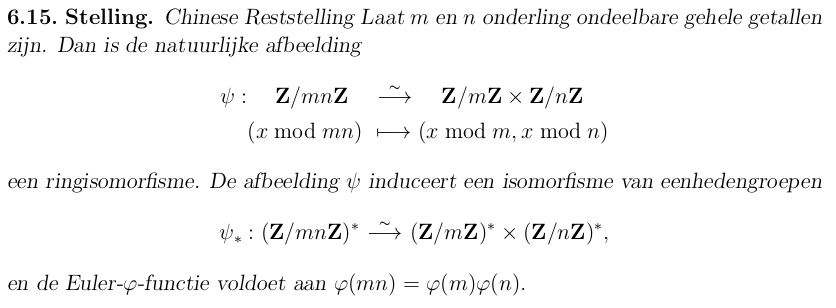
\includegraphics[width=\textwidth]{Selection_259}\\
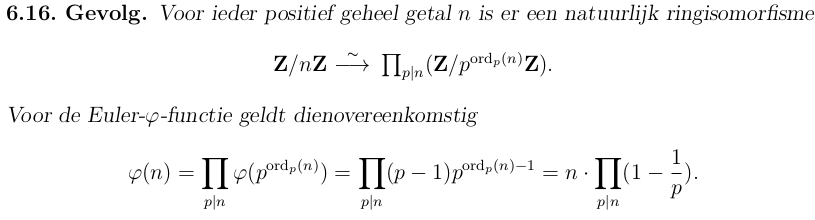
\includegraphics[width=\textwidth]{Selection_260}\\
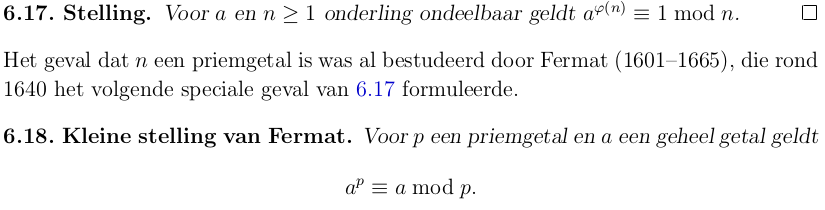
\includegraphics[width=\textwidth]{Selection_261}\\

\iffalse
\begin{center}
\begin{lstlisting}[frame=single, numbers=none, deletekeywords={for}]
~$ ku
ku: Permission denied, are you root?
~$ sudo ku
[sudo] password for root:
+-------+-------+-------+
| . . 7 | 1 . 6 | 3 . . | 
| . 1 . | 9 . 4 | . 5 . | 
| 8 . . | . . . | . . 4 | 
+-------+-------+-------+    
| . . 9 | 8 3 7 | 5 . . |    
| . . . | . . . | . . . | 
| . . 8 | 4 9 2 | 6 . . | 
+-------+-------+-------+
| 4 . . | . . . | . . 8 |
| . 5 . | 7 . 8 | . 3 . |
| . . 1 | 6 . 9 | 7 . . |
+-------+-------+-------+ 
\end{lstlisting}
\end{center}
\fi

\vfill
\begin{center}
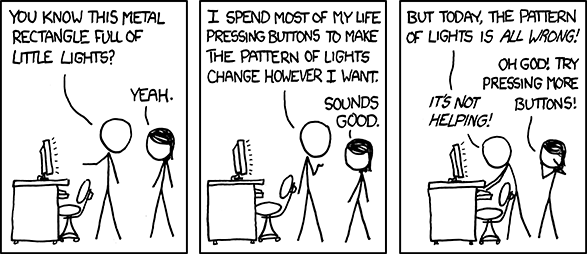
\includegraphics[height=150px]{XKCD0722.png}
\end{center}

\end{document}
